\documentclass[12pt]{article}

\usepackage[OT4]{polski}
\usepackage[utf8]{inputenc}
\usepackage{indentfirst}
\usepackage[left=2cm,right=2cm,top=1.5cm,bottom=2cm,includeheadfoot,a4paper]{geometry}
\usepackage{tabularx}
\usepackage{graphicx}
\usepackage{marginnote}
\usepackage{hyperref}
\usepackage{listings}

\usepackage[OT4]{polski}
\geometry{a4paper}
\linespread{1.25}
\frenchspacing
\graphicspath{ {./img/} }

\title{
	\huge{Państwowa Wyższa Szkoła Zawodowa \\ im. Witelona w Legnicy} \\
	\vspace{2cm}
	\Huge{Sprawozdanie z projektu grupowego aplikacji internetowej ,,PizzaOrders''} \\
	\vspace{1cm}
	\Large{Projektowanie i programowanie systemów internetowych II} \\
	\vspace{5mm}
	\Large{Prowadzący:} \\
	mgr inż. Krzysztof Rewak
	\vspace{1cm}
	\begin{flushright}
	Konrad Faliński \\ Filip Fonał \\ Mateusz Lencki \\ Adam Pankiewicz \\
	\vspace{1cm}
	Informatyka \\ Programowanie aplikacji mobilnych i internetowych
	\end{flushright}
}


\begin{document}

\maketitle

\section{Opis funkcjonalny}
\vspace{1cm}
Pizza orders to platforma internetowa przeznaczona dla restauracji typu pizzeria i ich klientów. Główną funkcjonalnością aplikacji jest graficzny kreator pizzy, w którym klient danej pizzerii może edytować już istniejące w menu rodzaje pizz lub może tworzyć całkowicie nowe kompozycje, wybierając odpowiednie pozycje z listy dostępnych w danej restauracji składników. Kreator pizzy ma postać edytora typu drag \& drop, w którym klient przeciąga składniki na ciasto na którym automatycznie jest  prezentowany końcowy wygląd tworzonej pizzy.

Oprócz kreatora pizzy aplikacja wspomaga proces zamawiania jedzenia w restauracji. Począwszy od złożenia zamówienia na stworzoną pizzę, poprzez odebranie zamówienia w kuchni, statusowanie przez kucharza postępów w przetwarzaniu zamówienia i skończywszy na dostarczeniu pizzy do klienta. Zmiany w statusach zamówienia są pokazywane klientowi w czasie rzeczywistym.

Właściciel pizzerii może zarejestrować swoją restauracje w aplikacji, dodać kucharzy i managerów magazynu. Jest możliwość zdefiniowania menu restauracji.
Po wypełnieniu wszystkich danych o restauracji można włączyć możliwość zamawiania pizzy przez klientów, zgłaszając tym samym zgłoszenie do administratora systemu aby ten opublikował naszą restauracje. Od momentu zatwierdzenia restauracji przez administratora jest ona widoczna w wyszukiwarce pizzerii a klienci mogą zamówić jedzenie.

Kolejną ważną funkcjonalnością jest panel zarządcy. Właściciel lub zarządca pizzerii ma dostęp do modułu, w którym można określać dostępność danych składników w restauracji i ich cenę. Składniki, które zostaną oznaczone jako dostępne są prezentowane końcowemu użytkownikowi w kreatorze pizzy. Mają one wtedy taką cene jaką ustali zarządca restauracji.

Następnym elementem systemu jest panel administracyjny, w którym osoba o szczególnych uprawnieniach może  zarządzać kluczowymi danymi w systemie takimi jak lista definicji składników pizzy, listy restauracji, użytkowników. Ma dostęp do logów i narzędzi analizy ruchu.

Na następnych stronach przedstawiono zrzuty najważniejszych ekranów systemu, które ukazują finalny wygląd aplikacji.
\clearpage

Główny widok aplikacji. Wyszukiwarka restauracji. \\

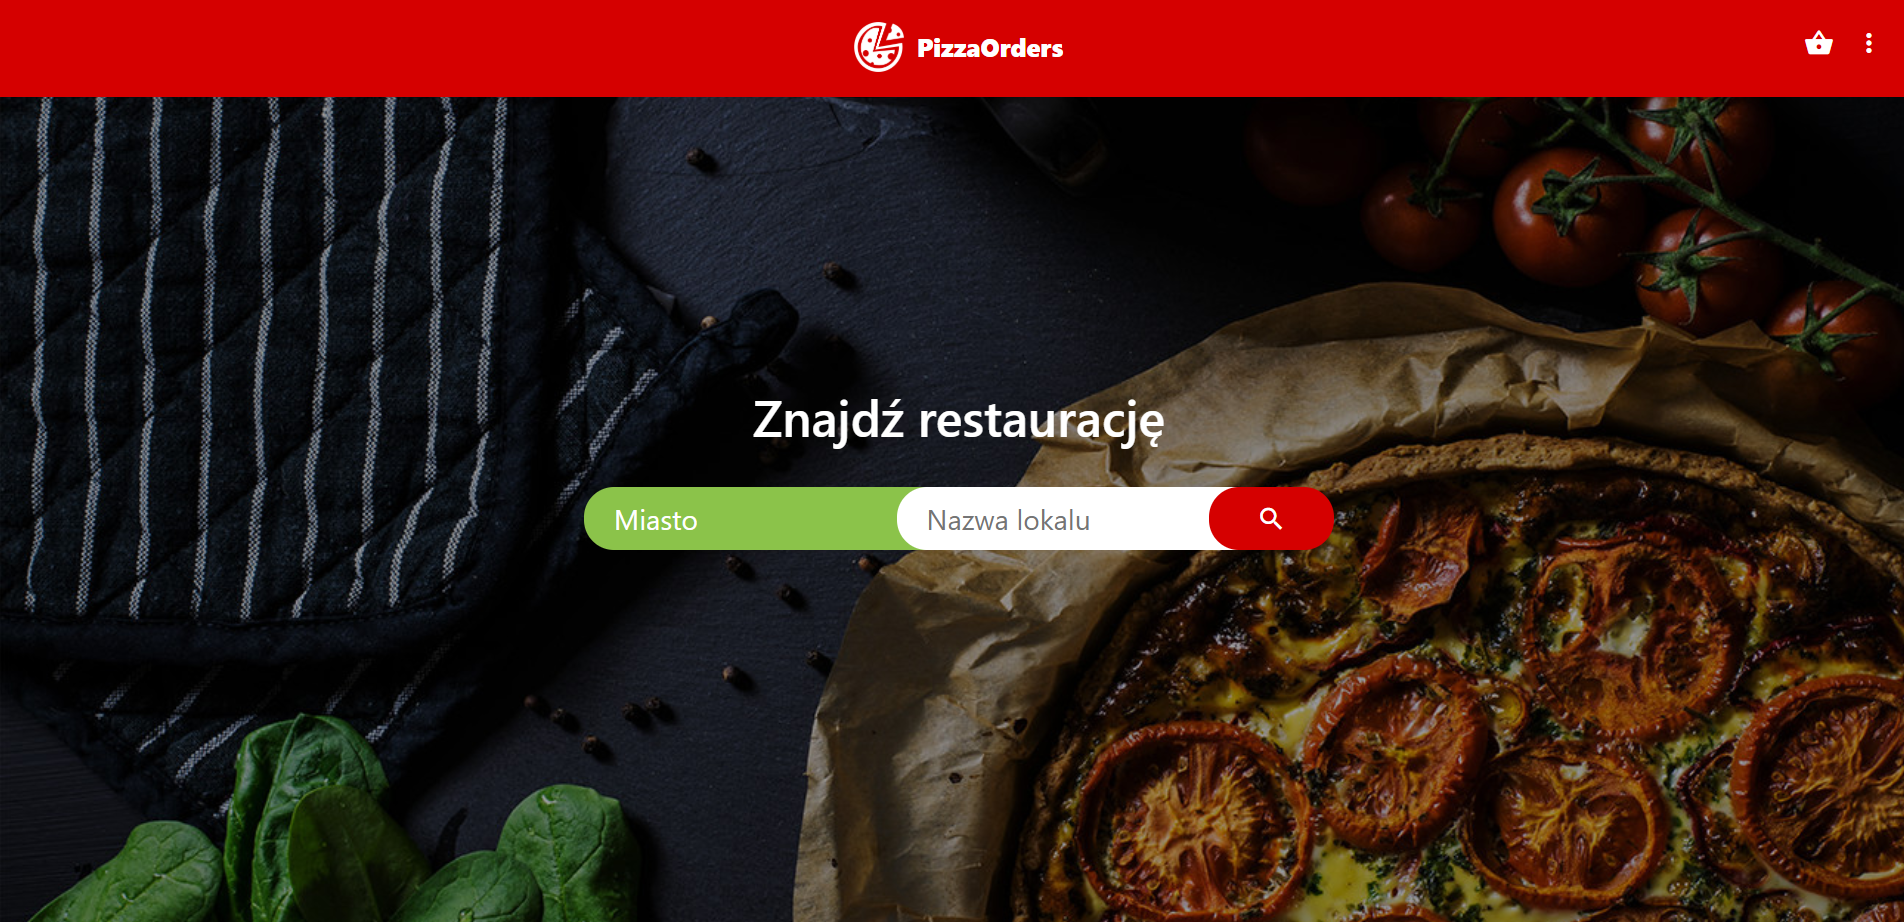
\includegraphics[width=16cm]{main}

\vspace{1cm}
Menu pojedynczej restauracji. \\

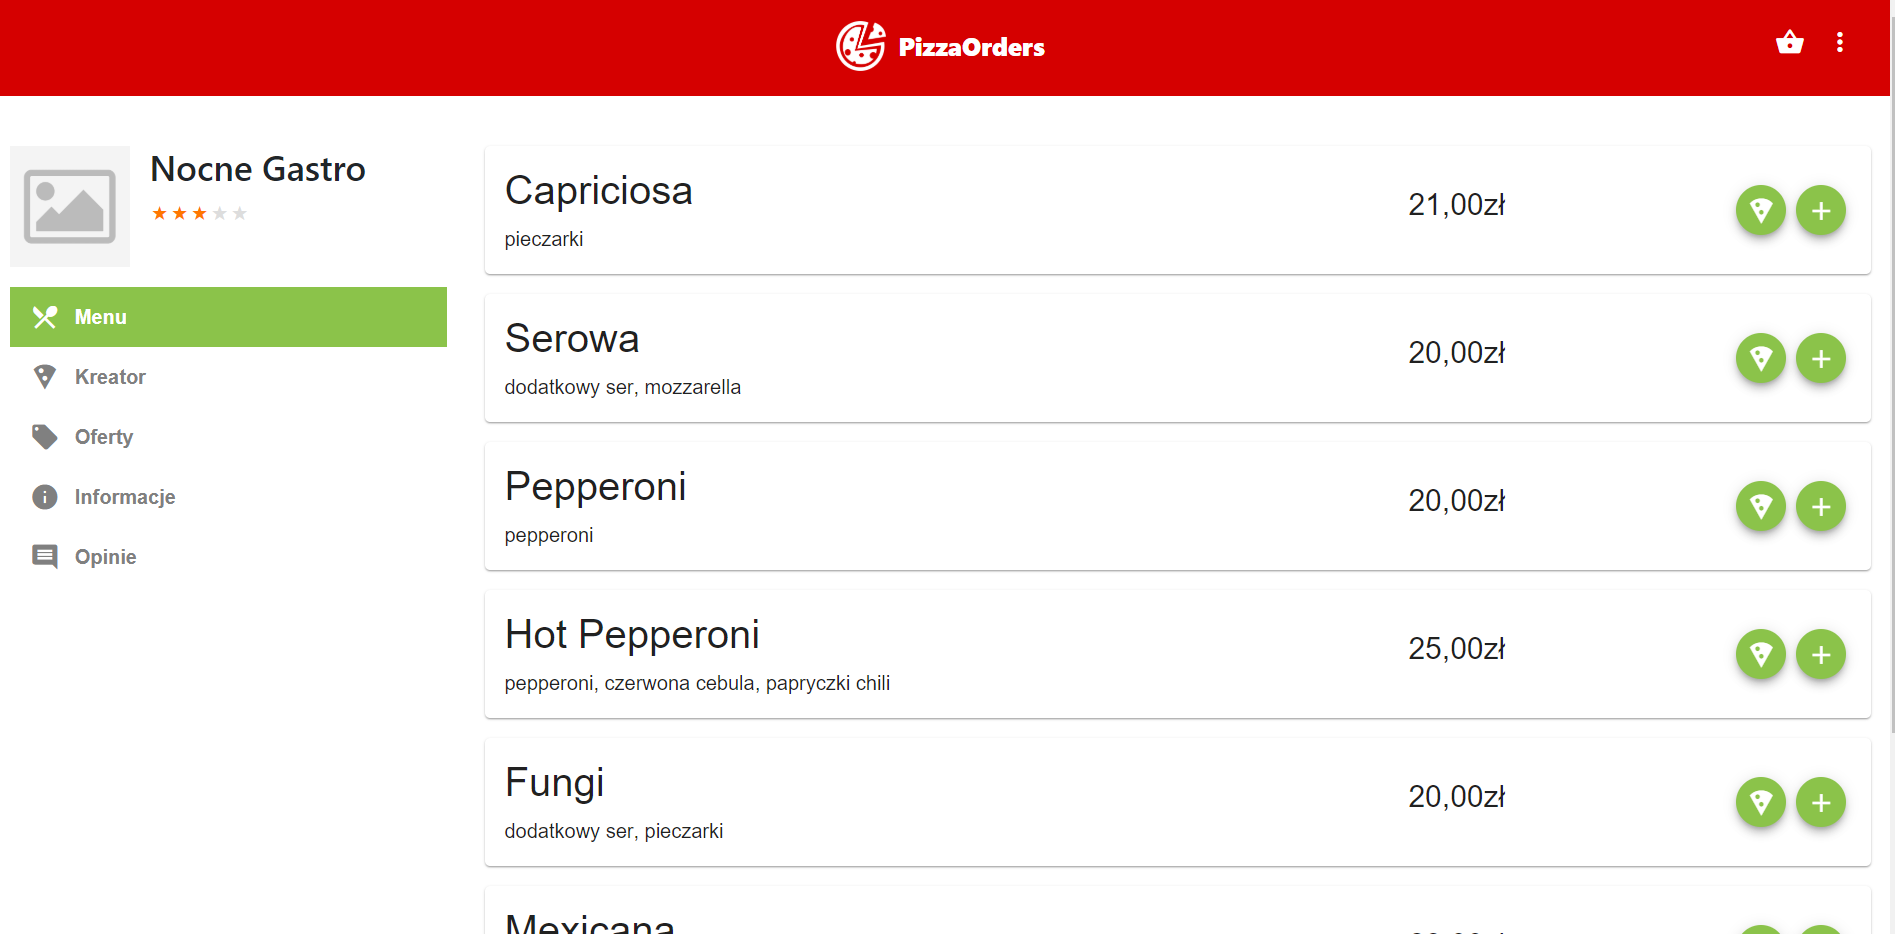
\includegraphics[width=16cm]{menu}

\clearpage

Kreator własnej pizzy. \\

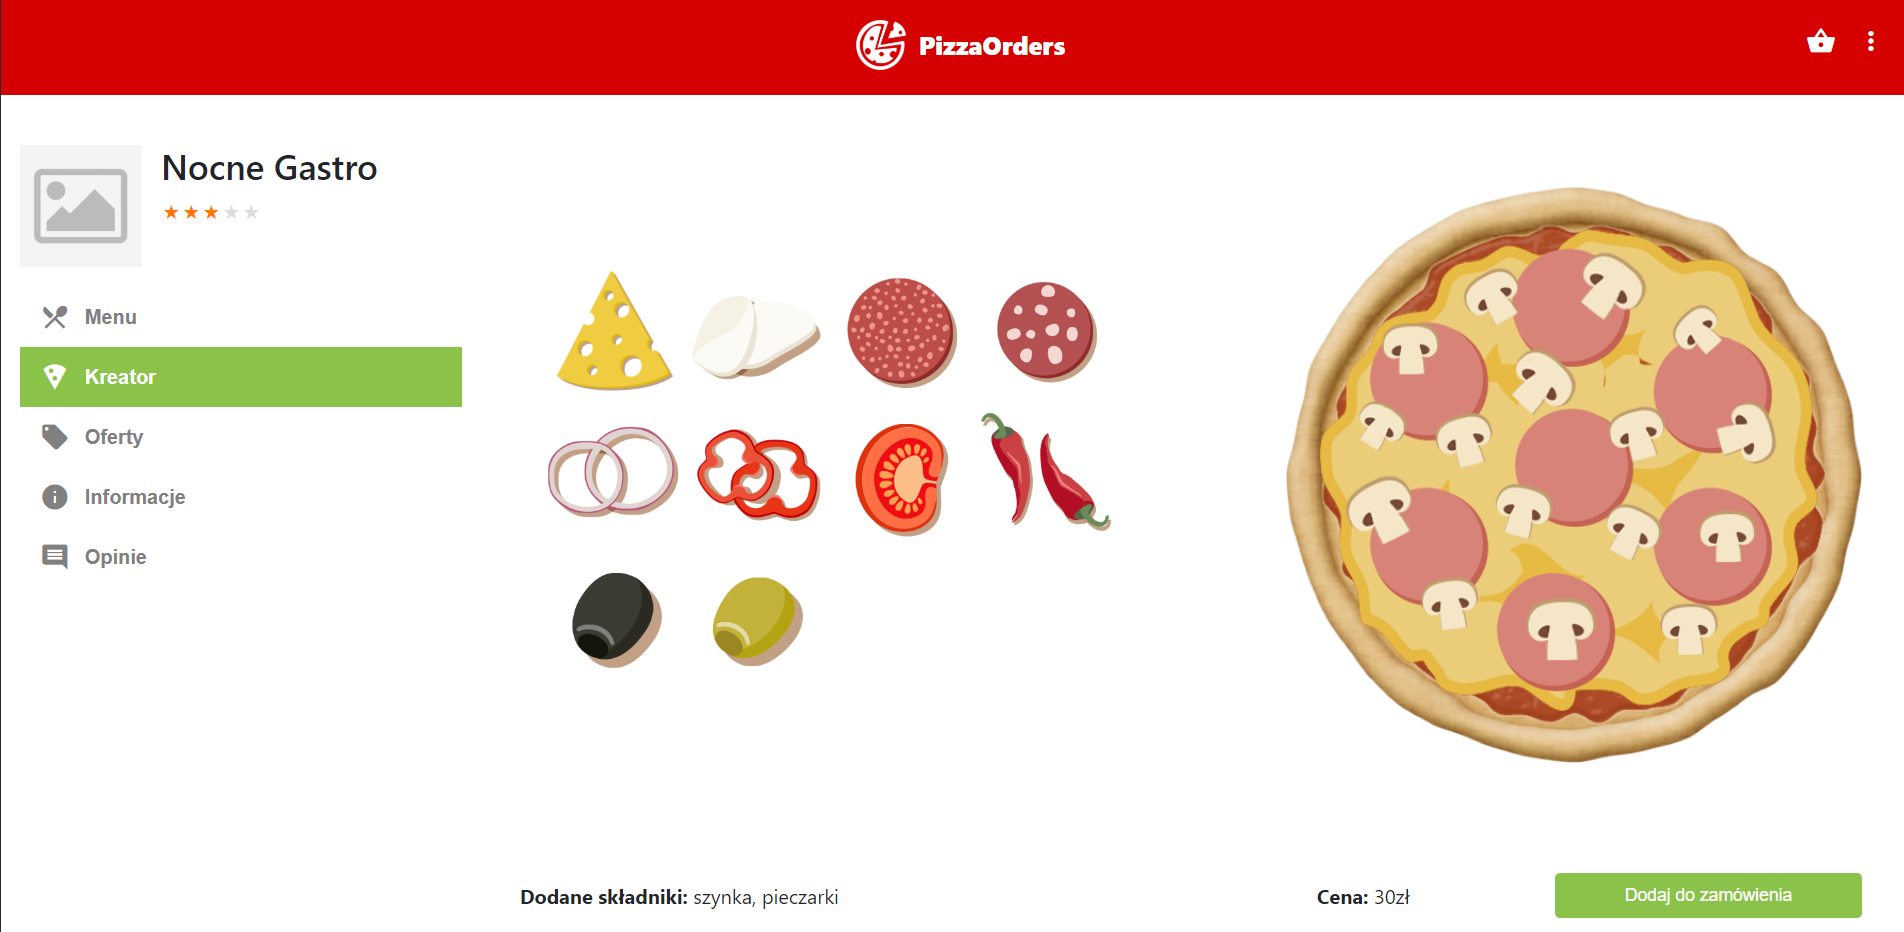
\includegraphics[width=16cm]{creator}

\vspace{1cm}

Widok ze śledzeniem zamówienia. \\

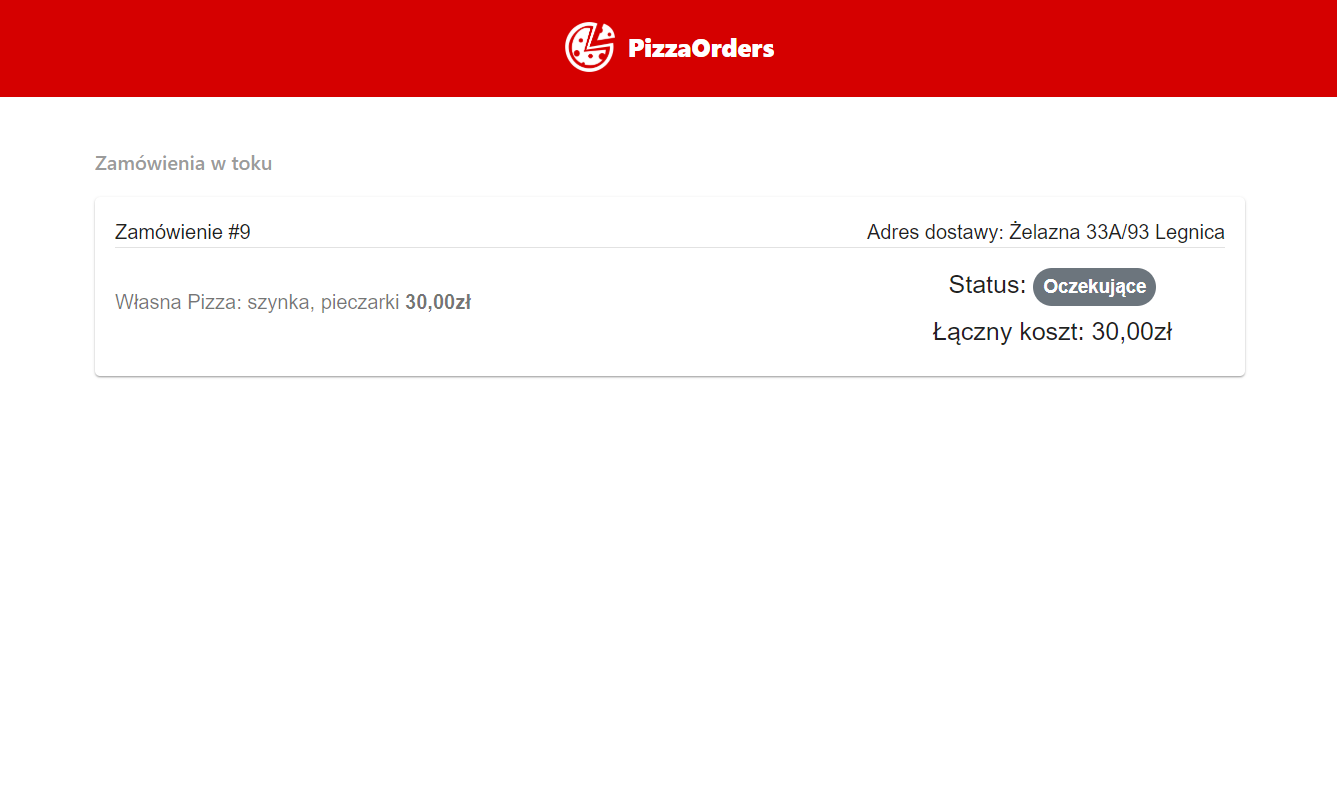
\includegraphics[width=16cm]{order}

\clearpage

Widok panelu kucharza z aktywnymi zamówieniami. \\

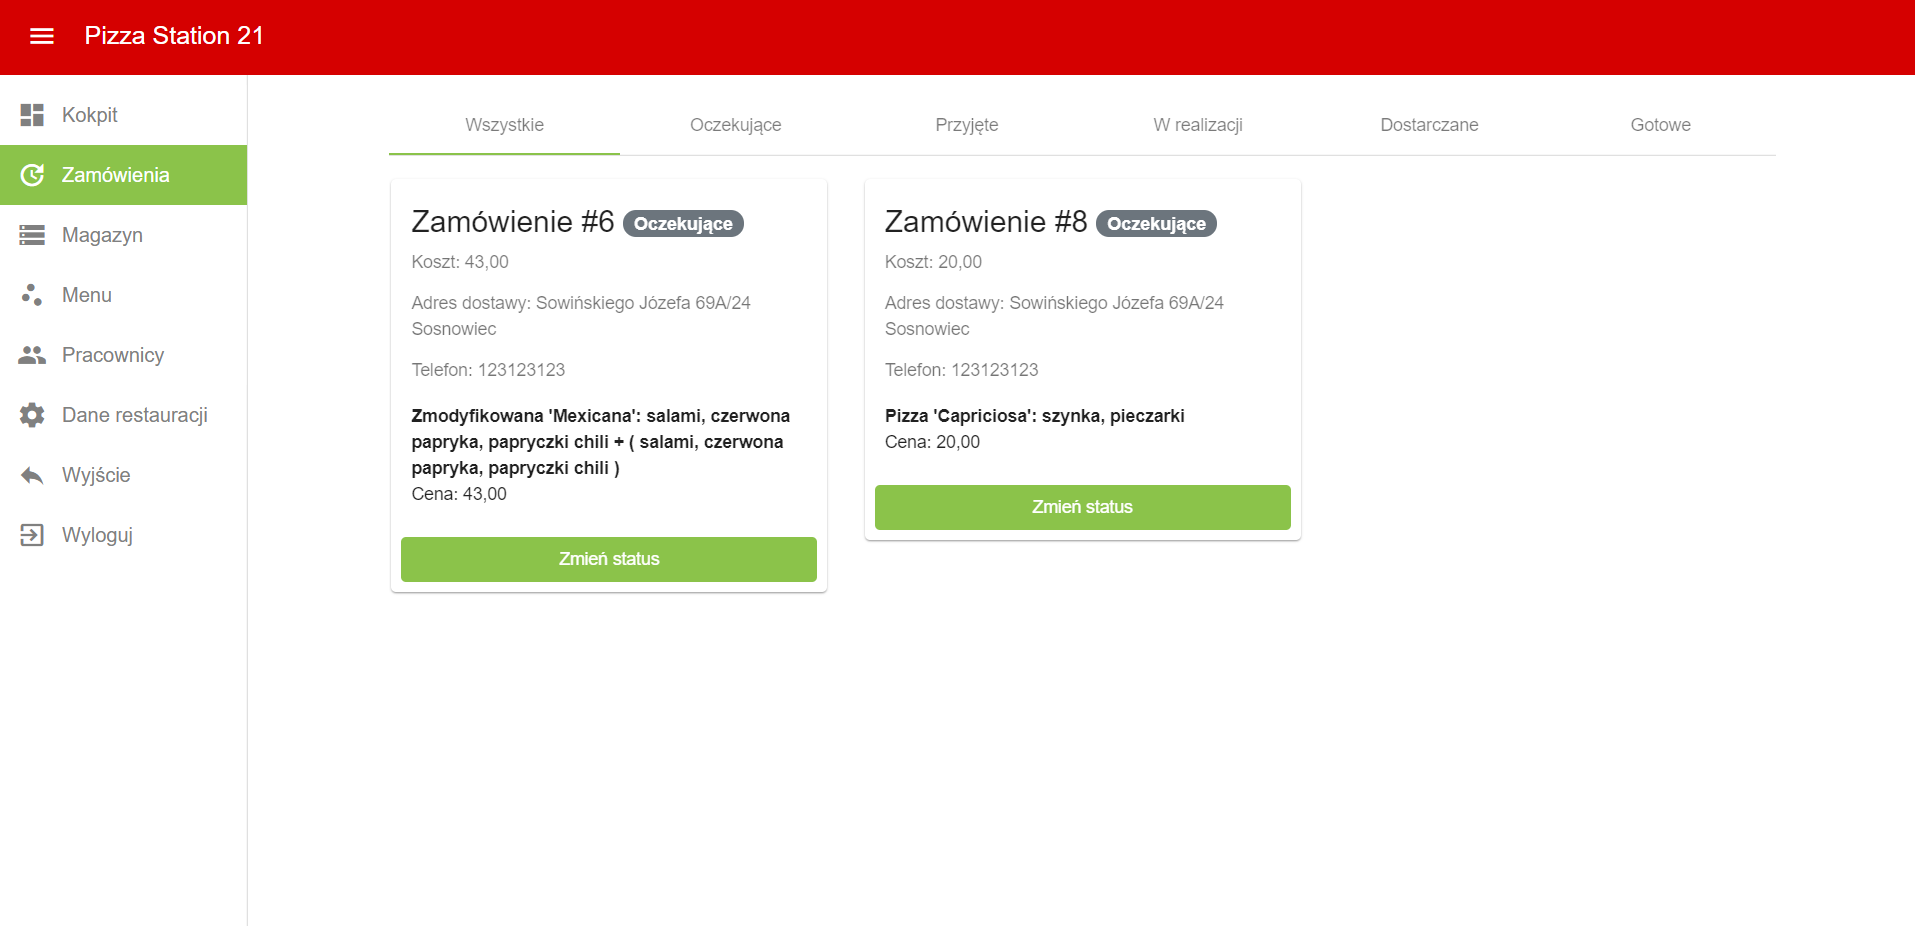
\includegraphics[width=16cm]{orders}

Widok zarządcy magazynu z dostępnymi składnikami. \\

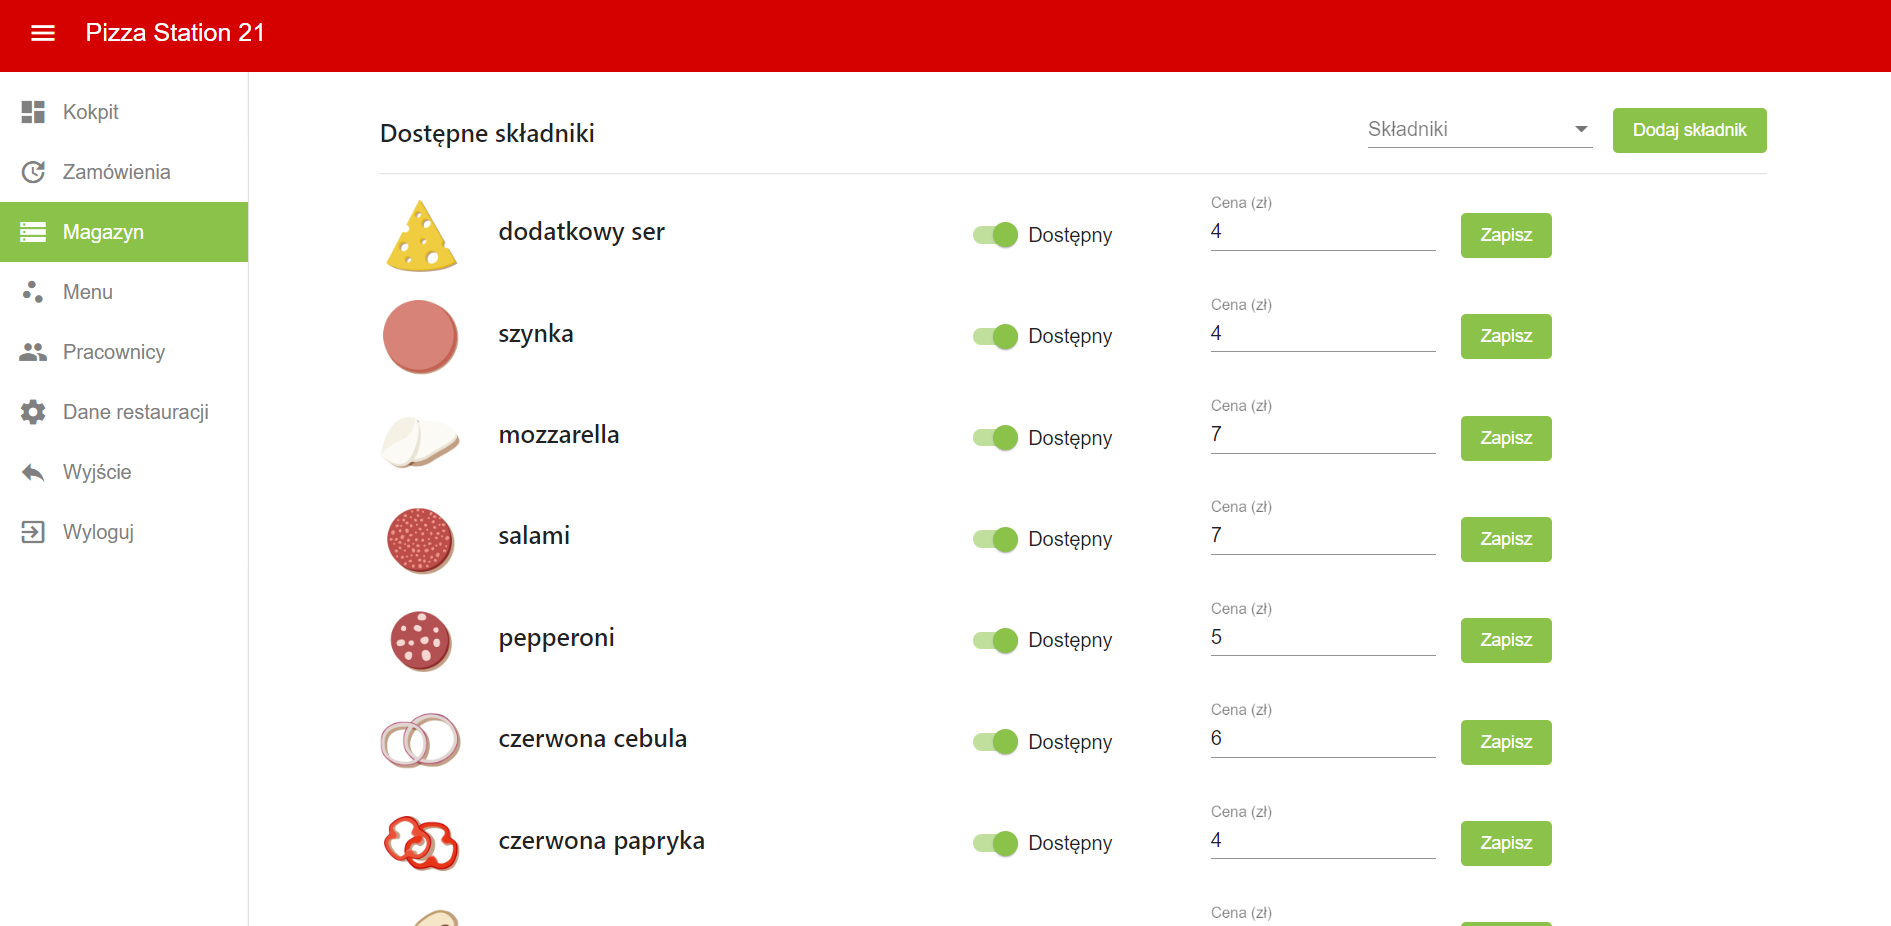
\includegraphics[width=16cm]{ingredients}

\clearpage

Panel administratora do zarządzania definicjami składników. \\

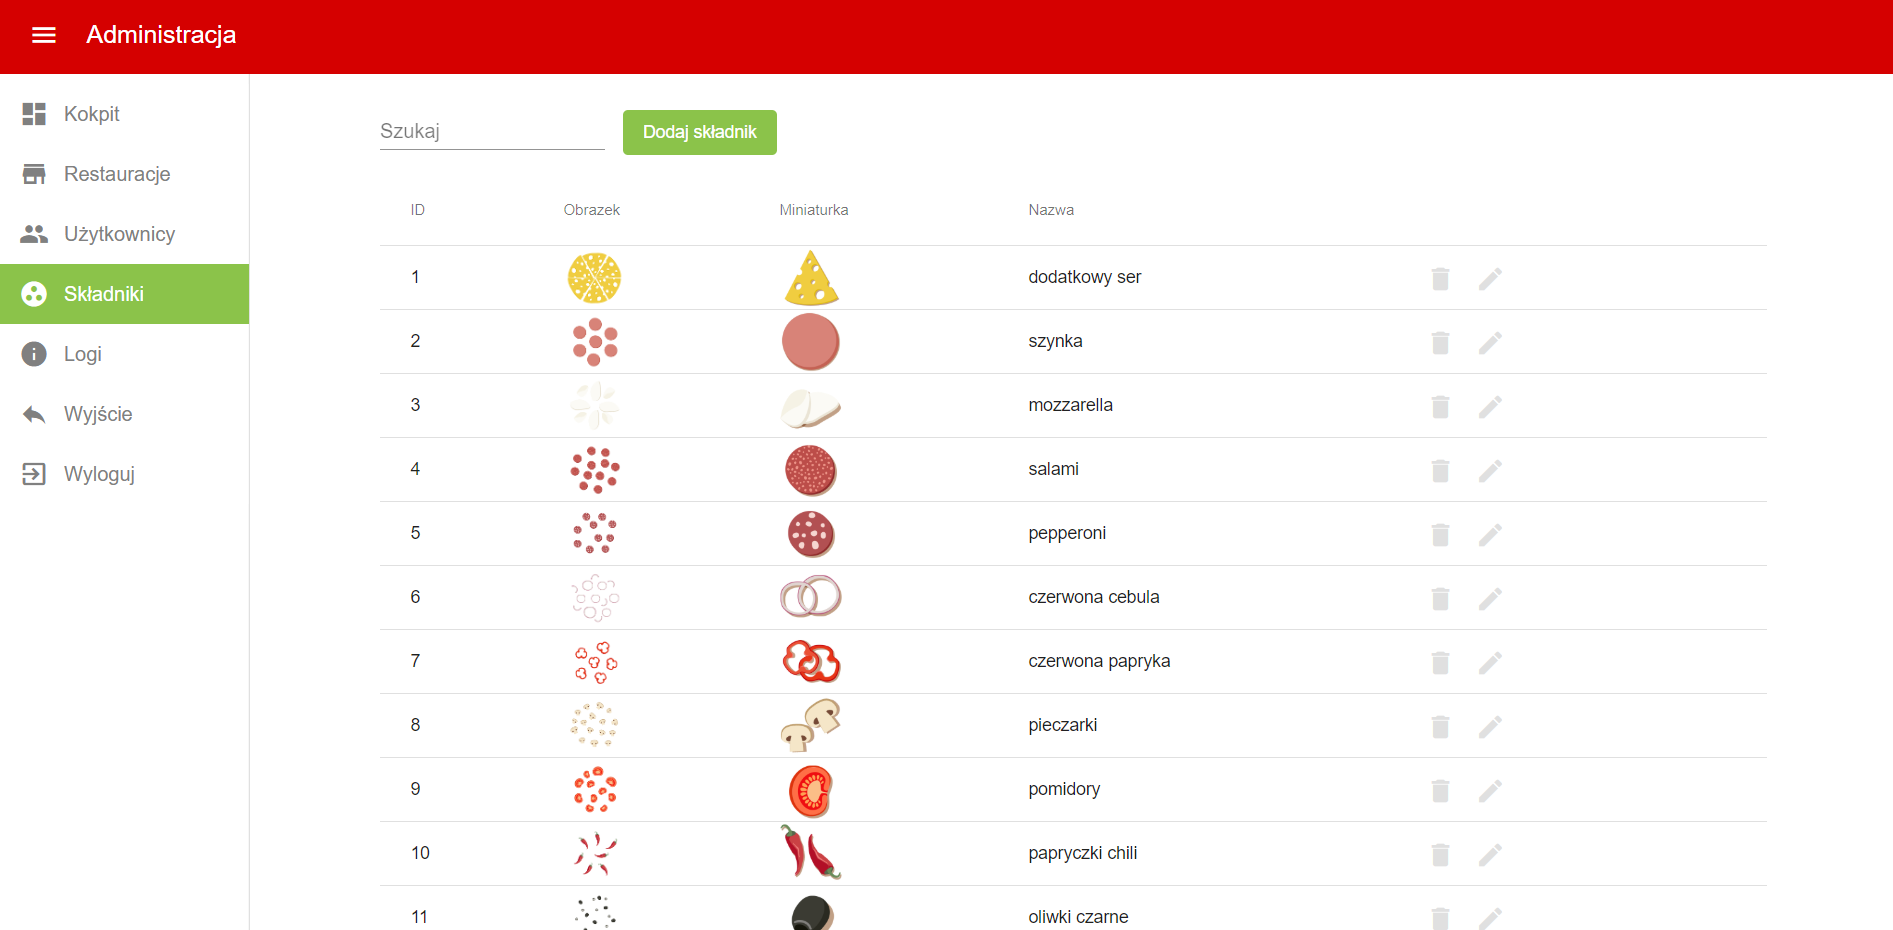
\includegraphics[width=16cm]{admin}

\clearpage
\vspace{1cm}
\section{Opis technologiczny}
\vspace{1cm}
Projekt jest zrealizowany w postaci aplikacji internetowej z wykorzystaniem różnorakich technologii internetowych.
Warstwa backendu i warstwa prezentacji to dwa osobne aplikacje, które wymieniają dane między sobą za pomocą udokumentowanego API. Dlatego też opis technologiczny można podzielić na dwie poniższe sekcje.

\subsection{Backend}

Backend aplikacji został zrealizowany z użyciem języka programowania PHP 7. Do innych technologii i narzędzi wykorzystanych w projekcie należą:
\begin{itemize}
	\item Laravel 5.7 - framework języka PHP.
	\item Baza danych MySQL.
	\item Pusher.
\end{itemize}

\subsection{Frontend}

Przy tworzeniu aplikacji frontendowej wykorzystano:
\begin{itemize}
	\item Angular 7.1.
	\item Material 7.2.
	\item Leaflet 1.3
\end{itemize}

\clearpage

\section{Instrukcja uruchomienia}
\vspace{1cm}
\subsection{Backend}

\begin{itemize}
	\item Pobranie projektu z repozytorium i pobranie zależności:
	\begin{lstlisting}[]
	git clone https://github.com/ppsi2-pizza-orders...
	.../pizza-orders-api
	\end{lstlisting}
	\begin{lstlisting}[]
	cd pizza-orders-api
	\end{lstlisting}
	\begin{lstlisting}[]
	composer install
	\end{lstlisting}
	\item Konfiguracja pliku .env:
	\begin{lstlisting}[]
	cp .env.example .env
	\end{lstlisting}
	W pliku .env należy ustawić odpowiednie dane dostępu do bazy danych itp.
	\begin{lstlisting}[]
	php artisan key:generate
	\end{lstlisting}
	\item Uruchomienie kontenerów dockerowych:
	\begin{lstlisting}[]
	docker-compose up -d
	\end{lstlisting}
	\item Migracja tabel w bazie danych i seed początkowych danych:
	\begin{lstlisting}[]
	php artisan migrate
	\end{lstlisting}
	\begin{lstlisting}[]
	php artisan db:seed
	\end{lstlisting}
	\item Wygenerowanie klucza JWT AUTH:
	\begin{lstlisting}[]
	php artisan jwt:secret
	\end{lstlisting}
	\item Aplikacja powinna być dostępna pod adresem:
	\begin{lstlisting}[]
	localhost:8080
	\end{lstlisting}
\end{itemize}

\clearpage

\subsection{Frontend}

\begin{itemize}
	\item Pobranie projektu z repozytorium:
	\begin{lstlisting}[]
	git clone https://github.com/ppsi2-pizza-orders...
	.../pizza-orders-frontend
	cd pizza-orders-frontend
	\end{lstlisting}
	\item Budowa kontnera dockerowego:
	\begin{lstlisting}[]
	docker-compose build
	\end{lstlisting}
	\item Uruchomienie aplikacji:
	\begin{lstlisting}[]
	docker-compose up
	\end{lstlisting}
	\item Budowanie aplikacji:
	\begin{lstlisting}[]
	docker exec -it pizza-orders-frontend bash
	ng build
	\end{lstlisting}
	\item Aplikacja jest dostępna pod adresem:
	\begin{lstlisting}[]
	localhost:4200
	\end{lstlisting}
\end{itemize}
\vspace{1cm}
\clearpage
\section{Instrukcja uruchomienia testów i opis testowanych \\ funkcjonalności}
\vspace{1cm}

Pisząc testy, skorzystaliśmy z narzędzia PHPUnit do testowania backendu naszej aplikacji.
Wiekszość z udokumentowanych endpointów została przetestowana za pomocą testów integracyjnych. Przetestowane zostały zarówno scenariusze domyślne jak i progowe, które powinny zostać odpowiednio obsłużone przez naszą aplikację.
W celu uruchomienia testów należy odpowiednio skonfigurować środowisko testowe.

\begin{itemize}
\item Należy skonfigurować plik .env.testing i ustawić w nim odpowiednie dostepy do bazy testowej:

\begin{lstlisting}[]
cp .env .env.testing
\end{lstlisting}

\item Migracja tabel do bazy testowej i uzupełnianie jej danymi testowymi:

\begin{lstlisting}[]
php artisan migrate --database=mysql_testing
php artisan db:seed --database=mysql_testing
\end{lstlisting}

\item Uruchomienie wszystkich testów:

\begin{lstlisting}[]
php vendor/phpunit/phpunit/phpunit
\end{lstlisting}

\end{itemize}

\clearpage

\section{Wnioski projektowe}
\vspace{1cm}
Odseparowanie backendu od warstwy prezentacji w postaci tworzenia dwóch oddzielnych aplikacji w projektach bardziej złożonych od najprostszych stron internetowych jest dobrym rozwiązaniem i rozsądnym podejściem do rozwijania nowoczesnych aplikacji internetowych. Takie rozwiązanie pozwala na lepszą koordynację prac między dwoma działami deweloperskimi zajmującymi się osobno wyglądem aplikacji i implementacją logiki biznesowej. Wymienianie danych w aplikacji za pomocą ustandaryzowanego i udokumentowanego API ułatwia pracę programistom frontendu jak i backendu. Człowiek odpowiedzialny za wygląd aplikacji, otrzymując dokumentację API nie musi zastanawiać się nad szczegółami implementacyjnymi funkcjonalności backendu i tak samo programista wnętrza systemu zwolniony jest z odpowiedzialności dostosowywania swojego kodu do wymagań frontendu. Podejście to pozwala również na połączenie innych aplikacji klienckich, takich jak np. aplikacja moblina, z już stworzonym API. 

Programowanie reaktywnych aplikacji frontendowych z użyciem różnorakich framework'ów, takich jak używany przez nas Angular, jest dużym ułatwieniem dla programisty. Korzystanie z gotowych mechanizmów zdarzeń, obserwatorów, dwustronnego wiązania zmiennych sprawia, że taka aplikacja powstaje szybciej w porównaniu do tradycyjnego podejścia stosowanego w przeszłości - ręcznego modyfikowania drzewa DOM dokumentu HTML za pomocą czystego języka JavaScript.

Stosowanie, już sprawdzonych wzorców i technik również pozwala na szybsze i łatwiejesze tworzenie zaawansowanych aplikacji internetowych. Wykorzystany przez nas PHP-owy framework Laravel implementuje szeroko stosowany wzorzec MVC - Model, View, Controller. Stawia on pewne ramy, których trzymanie się ułatwia pisanie kodu wysokiej jakości. Dzięki stosowaniu paradygmatu Inversion of Control, który implementujemy stosując wstrzykiwanie odpowiednich zależności do uzywanych przez nas klas, zwiększa modularność i skalowalność całości tworzonej aplikacji.

\clearpage

\section{Linki.}
\vspace{1cm}

Opublikowana aplikacja:

\url{https://pizzaorders.pl/}

\vspace{1cm}

Repozytoria projektu:

\url{https://github.com/ppsi2-pizza-orders}

\vspace{1cm}

Dokumentacjia API:

\url{https://api.pizzaorders.pl/api/documentation}

\end{document}
